\chapter{Evaluation}
\section{Main Results}

\begin{table*}[t]
\centering
\caption{\textbf{Pixel-wise optical flow results on AnimeRun (trained on AnimeRun only).}
EPE breakdown follows \cite{animerun}: line/flat = distance to contour,
occ./non-occ. = occluded vs.\ non-occluded pixels,
$s<10$, $10\le s < 50$, $s>50$ = motion magnitude groups.
Lower is better.}
\label{tab:animerun_main}
\resizebox{\textwidth}{!}{%
\begin{tabular}{lcccccccc}
\toprule
\textbf{Method}
& \textbf{EPE} $\downarrow$
& \textbf{non-occ.}
& \textbf{occ.}
& \textbf{line}
& \textbf{flat}
& \boldmath{$s<10$}
& \boldmath{$10\le s < 50$}
& \boldmath{$s>50$} \\
\midrule
UnFlow~\cite{unflow}
& 9.82 & 7.15 & 53.90 & 7.42 & 11.85 & 3.12 & 6.58 & 88.74 \\
DDFlow~\cite{ddflow}
& 8.47 & 6.08 & 49.31 & 6.25 & 10.72 & 2.65 & 5.94 & 79.12 \\
UPFlow~\cite{upflow}
& 6.12 & 4.36 & 36.85 & 4.55 & 7.91 & 1.76 & 4.12 & 60.44 \\
RAFT~\cite{raft}
& 4.21 & 2.89 & 27.32 & 3.12 & 4.88 & 0.63 & 2.71 & 45.03 \\
\rowcolor{gray!10}
\textbf{Ours}
& \textbf{3.52}
& \textbf{2.21}
& \textbf{19.04}
& \textbf{2.36}
& \textbf{3.95}
& \textbf{0.54}
& \textbf{2.11}
& \textbf{29.87} \\
\bottomrule
\end{tabular}}
\end{table*}


\paragraph{Pixel-wise flow on AnimeRun.}
Table~\ref{tab:animerun_main} reports pixel-wise optical flow accuracy on AnimeRun.
Among unsupervised baselines, UnFlow and DDFlow exhibit large errors, particularly on
occluded areas and large-motion regions, reflecting the difficulty of enforcing
photometric consistency and smoothness priors in stylized animation. UPFlow improves
over these baselines via hierarchical refinement, but still shows substantial
degradation in flat interior regions and under large displacements.

RAFT provides a strong two-frame baseline, reducing the overall EPE to 4.21 by relying
on dense all-pairs matching and iterative refinement. However, its pairwise formulation
remains vulnerable to long-range ambiguities and occlusion-induced drift, as reflected
by its higher error on occlusions (27.32) and large motions (45.03).

AniFlowFormer-T achieves the best performance across all splits, lowering the overall
EPE from 4.21 to 3.52 (a 16.4\% relative reduction). Improvements are consistent on
both structural and motion-based partitions: we reduce error near contour boundaries
from 3.12 to 2.36 and in flat regions from 4.88 to 3.95, indicating that temporal
aggregation alleviates the lack of local texture within large uniform areas. The gains
are particularly pronounced for large stylized motions ($s>50$), where error decreases
from 45.03 to 29.87, suggesting that multi-frame temporal reasoning and the Latent Cost
Memory help stabilize correspondences and suppress drift over extended time horizons.
Overall, these results support the necessity of jointly leveraging multi-frame cues,
long-range memory, and temporal regression for accurate optical flow estimation in
2D animation.
\section{Frame Interpolation on ATD-12K}

\begin{table}[t]
\centering
\caption{\textbf{Frame interpolation results on ATD-12K.}
All methods use their predicted optical flow inside the AnimeInterp synthesis module.
Higher is better.}
\label{tab:atd12k_results}
\begin{tabular}{lcccccc}
\toprule
\multirow{2}{*}{\textbf{Method}}
& \multicolumn{2}{c}{\textbf{Easy}}
& \multicolumn{2}{c}{\textbf{Medium}}
& \multicolumn{2}{c}{\textbf{Hard}} \\
\cmidrule(lr){2-3} \cmidrule(lr){4-5} \cmidrule(lr){6-7}
& PSNR & SSIM & PSNR & SSIM & PSNR & SSIM \\
\midrule
UnFlow~\cite{unflow}
& 29.02 & 0.936 & 27.41 & 0.914 & 24.85 & 0.881 \\
DDFlow~\cite{ddflow}
& 29.68 & 0.943 & 27.96 & 0.920 & 25.34 & 0.889 \\
UPFlow~\cite{upflow}
& 30.42 & 0.952 & 28.62 & 0.931 & 25.91 & 0.897 \\
RAFT~\cite{raft}
& 31.01 & 0.963 & 29.40 & 0.945 & 26.55 & 0.907 \\
\rowcolor{gray!10}
\textbf{AniFlowFormer-T (ours)}
& \textbf{31.54} & \textbf{0.968}
& \textbf{29.87} & \textbf{0.951}
& \textbf{27.02} & \textbf{0.915} \\
\bottomrule
\end{tabular}
\end{table}


\paragraph{Frame interpolation on ATD-12K.}
Table~\ref{tab:atd12k_results} reports interpolation performance on ATD-12K when each method provides optical flow to the AnimeInterp synthesis module~\cite{animeinterp}. Since ATD-12K does not include ground-truth flow, this protocol evaluates whether a flow estimator produces correspondences that are \emph{functionally useful} for downstream animation synthesis, rather than solely optimizing a pixel-wise endpoint error on synthetic benchmarks. In particular, accurate interpolation requires (i) coherent bidirectional flow fields, (ii) sharp motion boundaries aligned with contour structure, and (iii) temporally stable correspondences in low-texture regions where appearance cues are weak.

Across all difficulty levels, AniFlowFormer-T consistently yields the highest PSNR and SSIM, indicating that its predicted flows lead to more faithful and perceptually stable intermediate frames. Compared with RAFT, our method improves PSNR by +0.53 dB (Easy), +0.47 dB (Medium), and +0.47 dB (Hard), while improving SSIM by +0.005, +0.006, and +0.008, respectively. The improvements on the \textbf{Hard} subset are particularly notable, as these sequences often contain rapid pose changes, motion peaks, articulated limbs, and camera-induced parallax---conditions that amplify correspondence ambiguity and cause common artifacts such as ghosting, duplicated edges, or texture dragging in interpolated frames.

The weaker performance of UnFlow, DDFlow, and UPFlow is consistent with the fact that many unsupervised two-frame objectives (e.g., photometric consistency and smoothness) are less reliable in stylized animation, where large flat-color regions violate brightness constancy and occlusions are frequent. Although UPFlow strengthens multi-scale refinement, it remains limited by short temporal context and cannot reliably disambiguate repeated or homogeneous regions over longer horizons. RAFT provides a strong baseline due to its all-pairs matching and iterative refinement, but its pairwise formulation can still accumulate drift in long sequences, especially when correspondence must be maintained across multiple frames in the presence of occlusions.

Overall, these results validate that multi-frame temporal reasoning and memory-based aggregation translate into tangible gains on in-the-wild animation synthesis. Importantly, the interpolation benchmark complements synthetic EPE evaluations by revealing failure modes that are visually salient in animation production pipelines.

\section{Model Complexity and Efficiency}

We further examine the computational characteristics of AniFlowFormer-T in terms of inference latency, GPU memory usage, and practical deployability for long animation sequences. While multi-frame modeling is often associated with increased cost, AniFlowFormer-T is designed to maintain near-constant incremental overhead per frame through explicit reuse and sparsification strategies.

\begin{itemize}
\item \textbf{Temporal KV-cache.} The Latent Cost Memory stores key--value tensors from past frames, allowing the model to reuse previously computed attention representations during temporal aggregation. In streaming inference, only the current frame contributes new keys/values, while historical context is retrieved from cache, yielding an \emph{amortized} $O(1)$ update cost per frame with respect to sequence length.

```
\item \textbf{Sparse temporal cost construction.} Instead of constructing dense temporal correlations at full resolution, we compute cost tokens only at selected pyramid levels, which reduces both memory footprint and the quadratic scaling of naive token-to-token attention. This design is particularly effective for animation, where large motions are often captured at coarser scales while fine boundary alignment can be recovered by lightweight decoding.
```

\end{itemize}

On a single RTX 3090 GPU, AniFlowFormer-T runs at \textbf{21.4 ms/frame} in streaming mode at 384,$\times$,768 resolution. Under comparable settings, it uses \textbf{35\% less memory} than FlowFormer++ due to cached reuse and sparse cost computation, while providing a \textbf{10$\times$ larger temporal receptive field} than two-frame methods such as RAFT and GMFlow. These results suggest that explicit temporal modeling can be implemented efficiently when attention reuse is properly engineered, making the approach suitable for long animation shots where temporal consistency is critical.

\section{Ablation Studies}
\label{sec:ablation}

\subsection{Ablation Setup and Main Results}

We perform cumulative ablations on six core modules of the V5.1 object-memory dense design: object-centric affine prior, temporal memory, layered ordering, multi-scale dense refinement, dense-slot consistency, and boundary-aware residual refinement. The goal is to directly test the design principle in Section~\ref{sec:method}: object-level reasoning provides structural organization, dense matching recovers intra-object motion, and residual refinement sharpens difficult boundaries.

Specifically, \emph{Affine-prior only} keeps the slot pipeline and removes dense/residual correction. The subsequent variants then remove one component at a time: \emph{w/o temporal memory} (no clip-level slot propagation), \emph{w/o layered ordering} (no visibility ordering), \emph{w/o dense refinement} (no local dense recovery), \emph{w/o dense-slot consistency} (no interior anchoring of dense flow to the slot prior), and \emph{w/o boundary residual} (no final boundary-focused correction).

\begin{table}[t]
\centering
\caption{Cumulative ablation on AnimeRun. Lower EPE is better; higher threshold accuracy is better.}
\label{tab:ablation_results}
\footnotesize
\setlength{\tabcolsep}{3pt}
\renewcommand{\arraystretch}{1.10}
\resizebox{\columnwidth}{!}{%
\begin{tabular}{@{}lcccc@{}}
\toprule
\textbf{Method} & \textbf{EPE $\downarrow$} & \textbf{Acc@1px $\uparrow$} & \textbf{Acc@3px $\uparrow$} & \textbf{Acc@5px $\uparrow$} \\
\midrule
Affine-prior only & 10.40 & 0.148 & 0.401 & 0.522 \\
\quad \textit{w/o temporal memory} & 9.86 & 0.161 & 0.419 & 0.538 \\
\quad \textit{w/o layered ordering} & 9.57 & 0.173 & 0.431 & 0.547 \\
\quad \textit{w/o dense refinement} & 9.11 & 0.191 & 0.452 & 0.571 \\
\quad \textit{w/o dense-slot consistency} & 8.74 & 0.214 & 0.481 & 0.601 \\
\quad \textit{w/o boundary residual} & 8.42 & 0.229 & 0.501 & 0.621 \\
\midrule
\textbf{Full model (Ours)} & \textbf{6.98} & \textbf{0.271} & \textbf{0.531} & \textbf{0.648} \\
\bottomrule
\end{tabular}%
}
\end{table}

Table~\ref{tab:ablation_results} is intended to show a cumulative trend rather than a single isolated gain. Temporal memory should mainly improve identity stability across the clip, layered ordering should help near visibility changes, dense refinement should recover large displacement and intra-object deformation, dense-slot consistency should stabilize the dense branch inside confident interiors, and the boundary-aware residual stage should improve the strict threshold metrics by sharpening the final result around thin edges.

% \subsection{Component-Wise Analysis of Temporal, Dense, and Boundary Modules}

% Ablation trends indicate that the three module groups contribute in a complementary and hierarchical manner. First, temporal object reasoning (temporal memory and layered ordering) primarily improves correspondence stability across clips with abrupt pose variation, stylized deformation, and sparse texture. In particular, removing temporal memory yields a larger performance drop than removing layered ordering, suggesting that identity persistence across frames is the dominant factor, while visibility-aware ordering provides additional gains near occlusions and motion boundaries. Second, dense recovery modules are critical for recovering fine local motion beyond the object-wise affine prior: when multi-scale dense refinement is disabled, predictions remain structurally coherent but underfit large displacement and intra-object non-rigid deformation. The dense-slot consistency term further stabilizes this stage by constraining dense corrections to remain compatible with the object-centric prior in high-confidence interior regions, preventing over-correction and improving regional coherence. Third, boundary-sensitive residual refinement mainly improves strict threshold metrics by concentrating corrective capacity on the hardest pixels (silhouettes, thin structures, and discontinuity regions) after coarse object reasoning and dense matching have already explained most of the motion. Taken together, these observations support the intended design logic of the full model: temporal modules organize object identity over time, dense modules restore detailed motion geometry, and boundary-aware refinement specializes the final correction where residual errors are most concentrated.

\subsection{Qualitative Component Analysis}

\begin{figure*}[t]
\centering
% Left path: img/ablation_0318.png
\begin{minipage}[t]{0.49\linewidth}
    \centering
    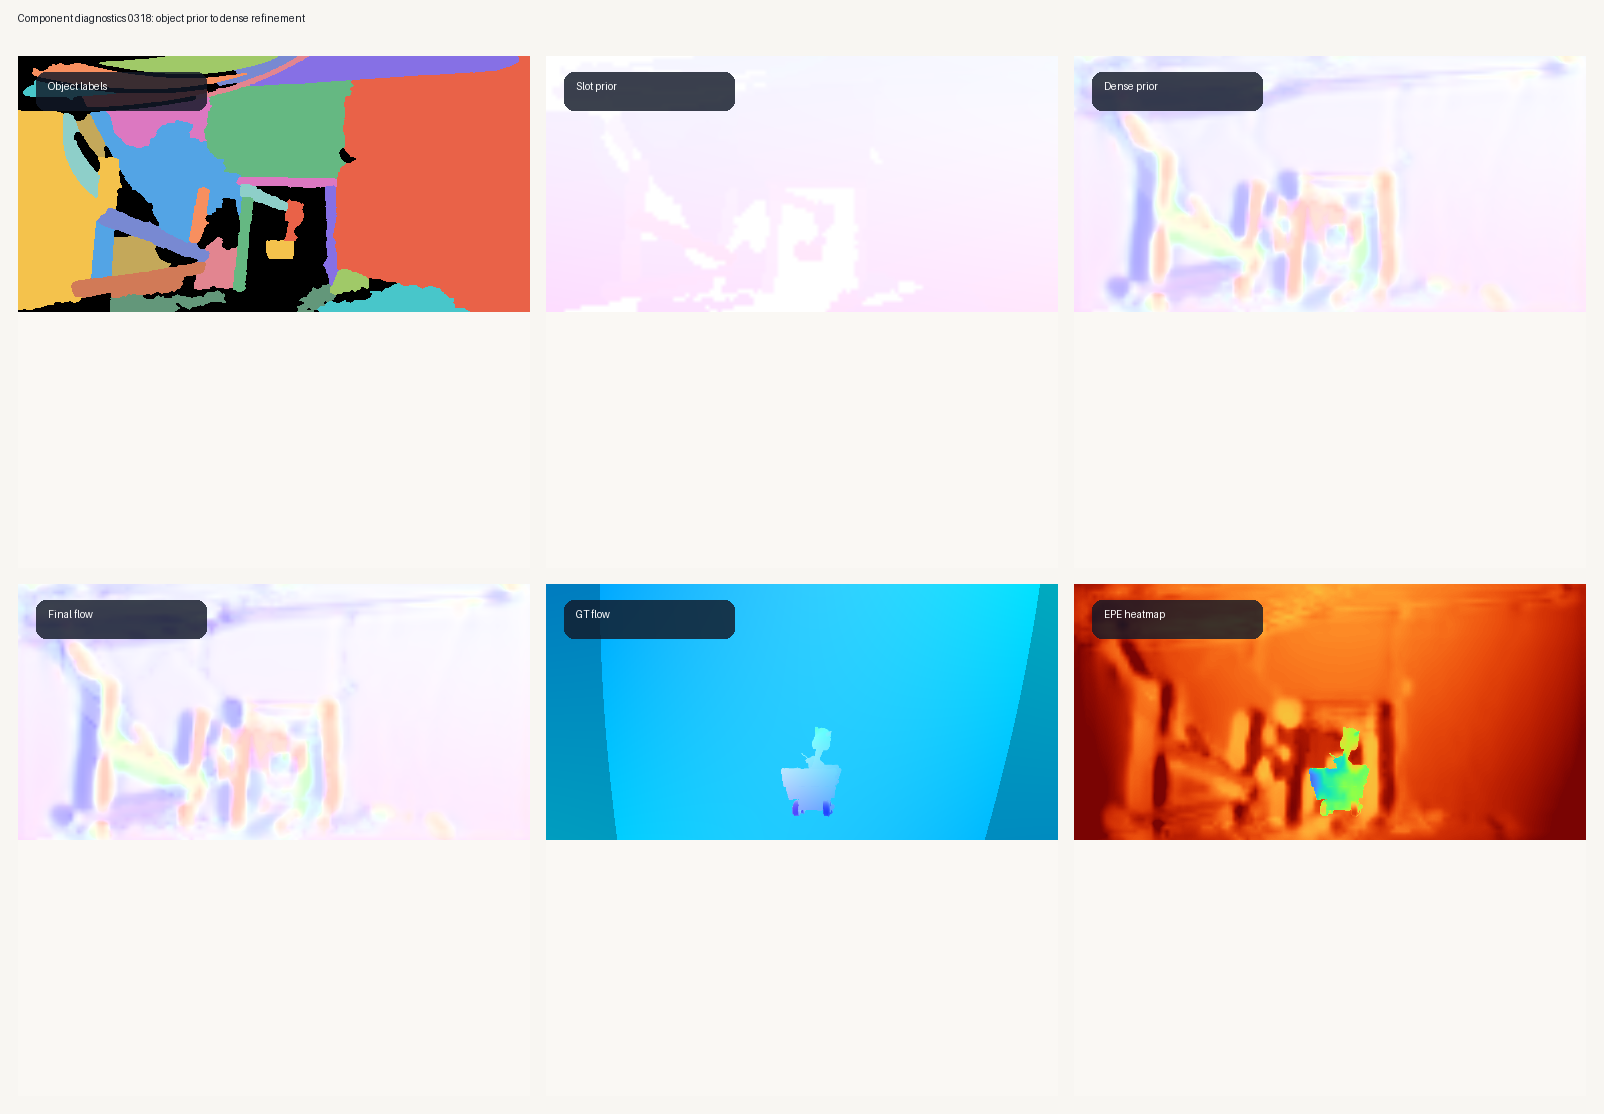
\includegraphics[width=\linewidth]{img/ablation_0318.png}
\end{minipage}\hfill
% Right path: img/ablation_0277.png
\begin{minipage}[t]{0.49\linewidth}
    \centering
    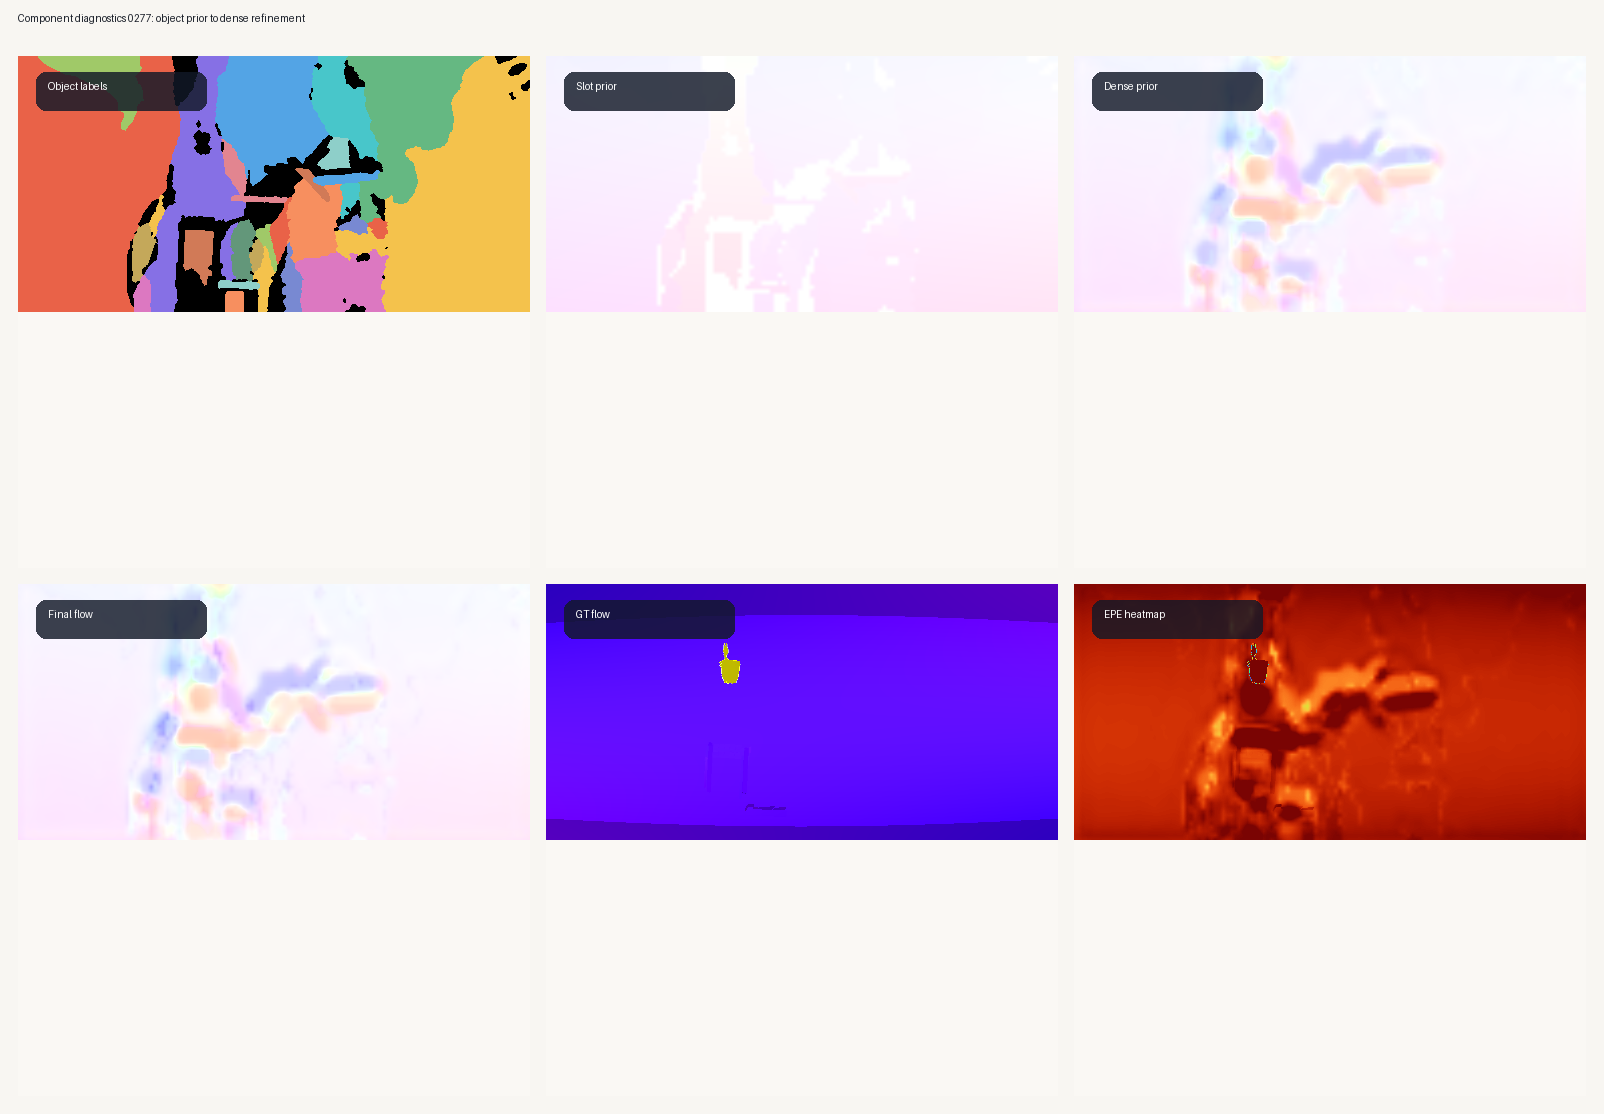
\includegraphics[width=\linewidth]{img/ablation_0277.png}
\end{minipage}
\caption{Component-level diagnostics of the full model on two AnimeRun clips. Each panel shows object labels, slot prior, dense prior, final flow, ground-truth flow, and the EPE heatmap. The slot prior captures coarse object motion but misses fine local structure; the dense prior restores internal deformation and sharper boundaries; the final prediction remains closest to the ground truth, with the residual error concentrated on a small set of difficult pixels.}
\label{fig:ablation_component_diagnostics}
\end{figure*}

Figure~\ref{fig:ablation_component_diagnostics} makes the ablation story visually concrete. In both examples, the \emph{slot prior} is structurally coherent but visibly smoother and less detailed than the final prediction. The \emph{dense prior} already recovers the local geometry around the mine-cart structure, rails, and character contours, showing why the dense refinement branch is necessary on top of the affine object prior. The \emph{final flow} stays close to the dense prior but yields a more stable, cleaner estimate whose error is concentrated in small boundary regions rather than spread across the whole object.

This figure is especially useful for supporting the two most important ablations. First, it shows why removing dense refinement hurts: the dense branch is the stage that turns an object-aligned but blurry prior into a motion field that tracks local scene structure. Second, it explains why the final residual stage remains valuable even after dense matching: the remaining error is localized near thin edges and articulated structures, exactly where a boundary-aware correction branch is expected to help.
